\appendix
%------------------------------------------------
\section{appendix}
%------------------------------------------------

\begin{frame}<1-4>{Detection Transformer (DETR)}

\tikzset{
  onslide/.code args={<#1>#2}{%
    \only<#1>{\pgfkeysalso{#2}}%
  }
}

\begin{columns}[T]
\begin{column}{0.45\textwidth}
    \centering
    \vspace{0.5cm}
    \begin{figure}
        \centering
        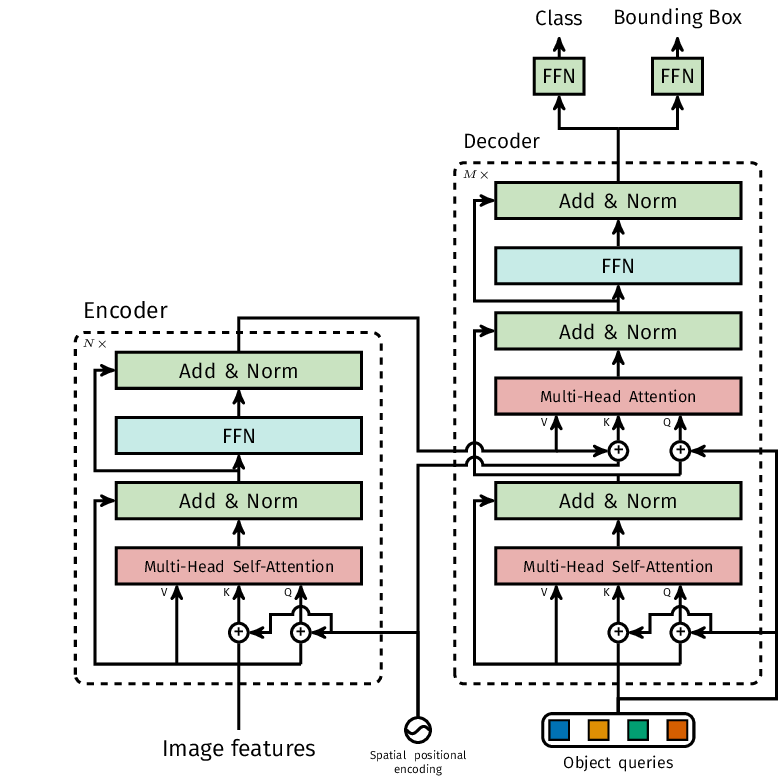
\includegraphics[width=0.95\linewidth]{detr.png}
        \caption{DETR architecture overview}
        \label{fig:detr_detailed}
    \end{figure}
\end{column}

\begin{column}{0.45\textwidth}
\only<1>{
\vspace{0.3cm}
\textbf{Step 1: Feature Extraction \& Positional Encoding}

\begin{block}{CNN Backbone}
\small
\textbf{ResNet-50 Feature Extraction:}
\begin{itemize}
\item Input: $\mathbf{x}_{img} \in \mathbb{R}^{H \times W \times 1}$
\item CNN features: $\mathbf{f} \in \mathbb{R}^{H/32 \times W/32 \times C}$
\item Lower resolution but rich semantics
\item $C = 2048$ for ResNet-50
\end{itemize}
\end{block}

\begin{block}{Positional Encoding}
\small
\textbf{Spatial Position Information:}
$$\mathbf{f}_{final} = \mathbf{f} + \mathbf{pos}$$
\begin{itemize}
\item Sine/cosine positional encoding
\item Essential for spatial reasoning
\item $\mathbf{pos} \in \mathbb{R}^{H/32 \times W/32 \times C}$
\item Enables transformer to understand spatial layout
\end{itemize}
\end{block}
}

\only<2>{
\vspace{0.3cm}
\textbf{Step 2: Transformer Encoder}

\begin{block}{Self-Attention Mechanism}
\small
\textbf{Multi-Head Self-Attention:}
$$\text{MSA}(\mathbf{X}) = \text{Concat}(\text{head}_1, ..., \text{head}_h)\mathbf{W}^O$$
$$\text{head}_i = \text{Attention}(\mathbf{X}\mathbf{W}_i^Q, \mathbf{X}\mathbf{W}_i^K, \mathbf{X}\mathbf{W}_i^V)$$
\textbf{Where:}
$$\text{Attention}(\mathbf{Q}, \mathbf{K}, \mathbf{V}) = \text{softmax}\left(\frac{\mathbf{Q}\mathbf{K}^T}{\sqrt{d_k}}\right)\mathbf{V}$$
\end{block}

\begin{block}{Encoder Layer Structure}
\small
$$\mathbf{z}_l = \text{MSA}(\text{LN}(\mathbf{z}_{l-1})) + \mathbf{z}_{l-1}$$
$$\mathbf{z}_l = \text{FFN}(\text{LN}(\mathbf{z}_l)) + \mathbf{z}_l$$
\begin{itemize}
\item Global receptive field from first layer
\item $N \times$ encoder layers process image features
\end{itemize}
\end{block}
}

\only<3>{
\vspace{0.3cm}
\textbf{Step 3: Transformer Decoder \& Object Queries}

\begin{block}{Object Queries}
\small
\textbf{Learnable Detection Slots:}
\begin{itemize}
\item $N = 100$ learnable embeddings
\item $\mathbf{q}_{obj} \in \mathbb{R}^{N \times d}$ (where $d = 256$)
\item Each query focuses on different objects
\item Learned during training to specialize
\end{itemize}
\textbf{Query Initialization:}
$$\mathbf{q}_{obj} \sim \mathcal{N}(0, \sigma^2)$$
\end{block}

\begin{block}{Decoder Layer}
\small
\textbf{Self-Attention + Cross-Attention:}
$$\mathbf{q}_l = \text{SelfAttn}(\text{LN}(\mathbf{q}_{l-1})) + \mathbf{q}_{l-1}$$
$$\mathbf{q}_l = \text{CrossAttn}(\text{LN}(\mathbf{q}_l), \mathbf{z}_{enc}) + \mathbf{q}_l$$
$$\mathbf{q}_l = \text{FFN}(\text{LN}(\mathbf{q}_l)) + \mathbf{q}_l$$
\end{block}
}

\only<4>{
\vspace{0.3cm}
\textbf{Step 4: Prediction \& Hungarian Matching}

\begin{block}{Prediction Heads}
\small
\textbf{Classification Head:}
$$p_i = \text{softmax}(\text{FFN}_{cls}(\mathbf{q}_i))$$
\textbf{Box Regression Head:}
$$\mathbf{b}_i = \sigma(\text{FFN}_{box}(\mathbf{q}_i))$$
\begin{itemize}
\item Each query produces one prediction
\end{itemize}
\end{block}
\vspace{-0.2cm}
\begin{block}{Hungarian Algorithm}
\small
\textbf{Bipartite Matching:}
$$\hat{\sigma} = \arg\min_{\sigma \in \mathfrak{S}_N} \sum_{i}^N \mathcal{L}_{match}(y_i, \hat{y}_{\sigma(i)})$$
\textbf{Set-based Loss:}
$$\mathcal{L} = \sum_{i=1}^N [-\log \hat{p}_{\hat{\sigma}(i)}(c_i) + \mathbbm{1}_{\{c_i \neq \emptyset\}} \mathcal{L}_{box}(b_i, \hat{b}_{\hat{\sigma}(i)})]$$
\end{block}
}

\end{column}
\end{columns}

\end{frame}

%--------

\begin{frame}{Data cleaning: Quality Assurance}
    \framesubtitle{Systematic Dataset Cleaning and Correction}
    
    The CBIS-DDSM dataset presented several critical inconsistencies requiring systematic correction
    
    \vspace{0.2cm}
    
     \textbf{Unnecessary Image Regions}
            \begin{itemize}
                \item Mammograms contained irrelevant background and metadata areas
                \item \textit{Solution:} Implemented cropping algorithm (provided by Mr. Yassine Ameskine) to isolate regions of interest
                \item \textit{Impact:} Focused processing on clinically relevant breast tissue only
            \end{itemize}
       \begin{figure}
                \centering
                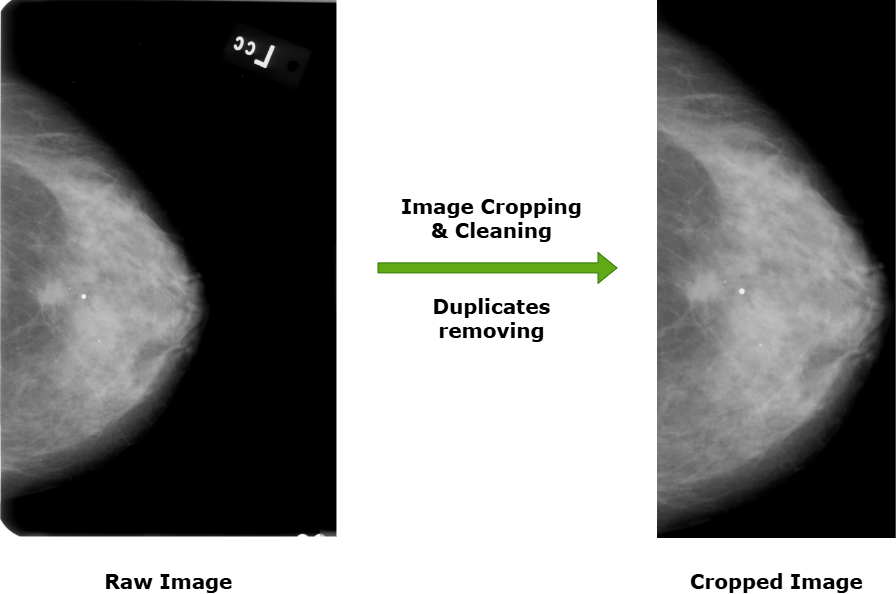
\includegraphics[width=0.4\linewidth]{preprocessing1.png}
        \end{figure}     
\end{frame}

\begin{frame}{Data cleaning: File Recovery}
    \framesubtitle{Addressing Corruption and Annotation Errors}
    
    
        \vspace{0.2cm}
        
        \textbf{File Corruption and Mismatched Annotations}
            \begin{itemize}
                \item Swapped filenames between masks and ROI files
                \item Missing or deleted mask files
                \item \textit{Solution:} Developed directory correction algorithm to restore proper file associations and recover masks from ROI
            \end{itemize}
        
        \vspace{0.2cm}
        \begin{figure}
            \centering
            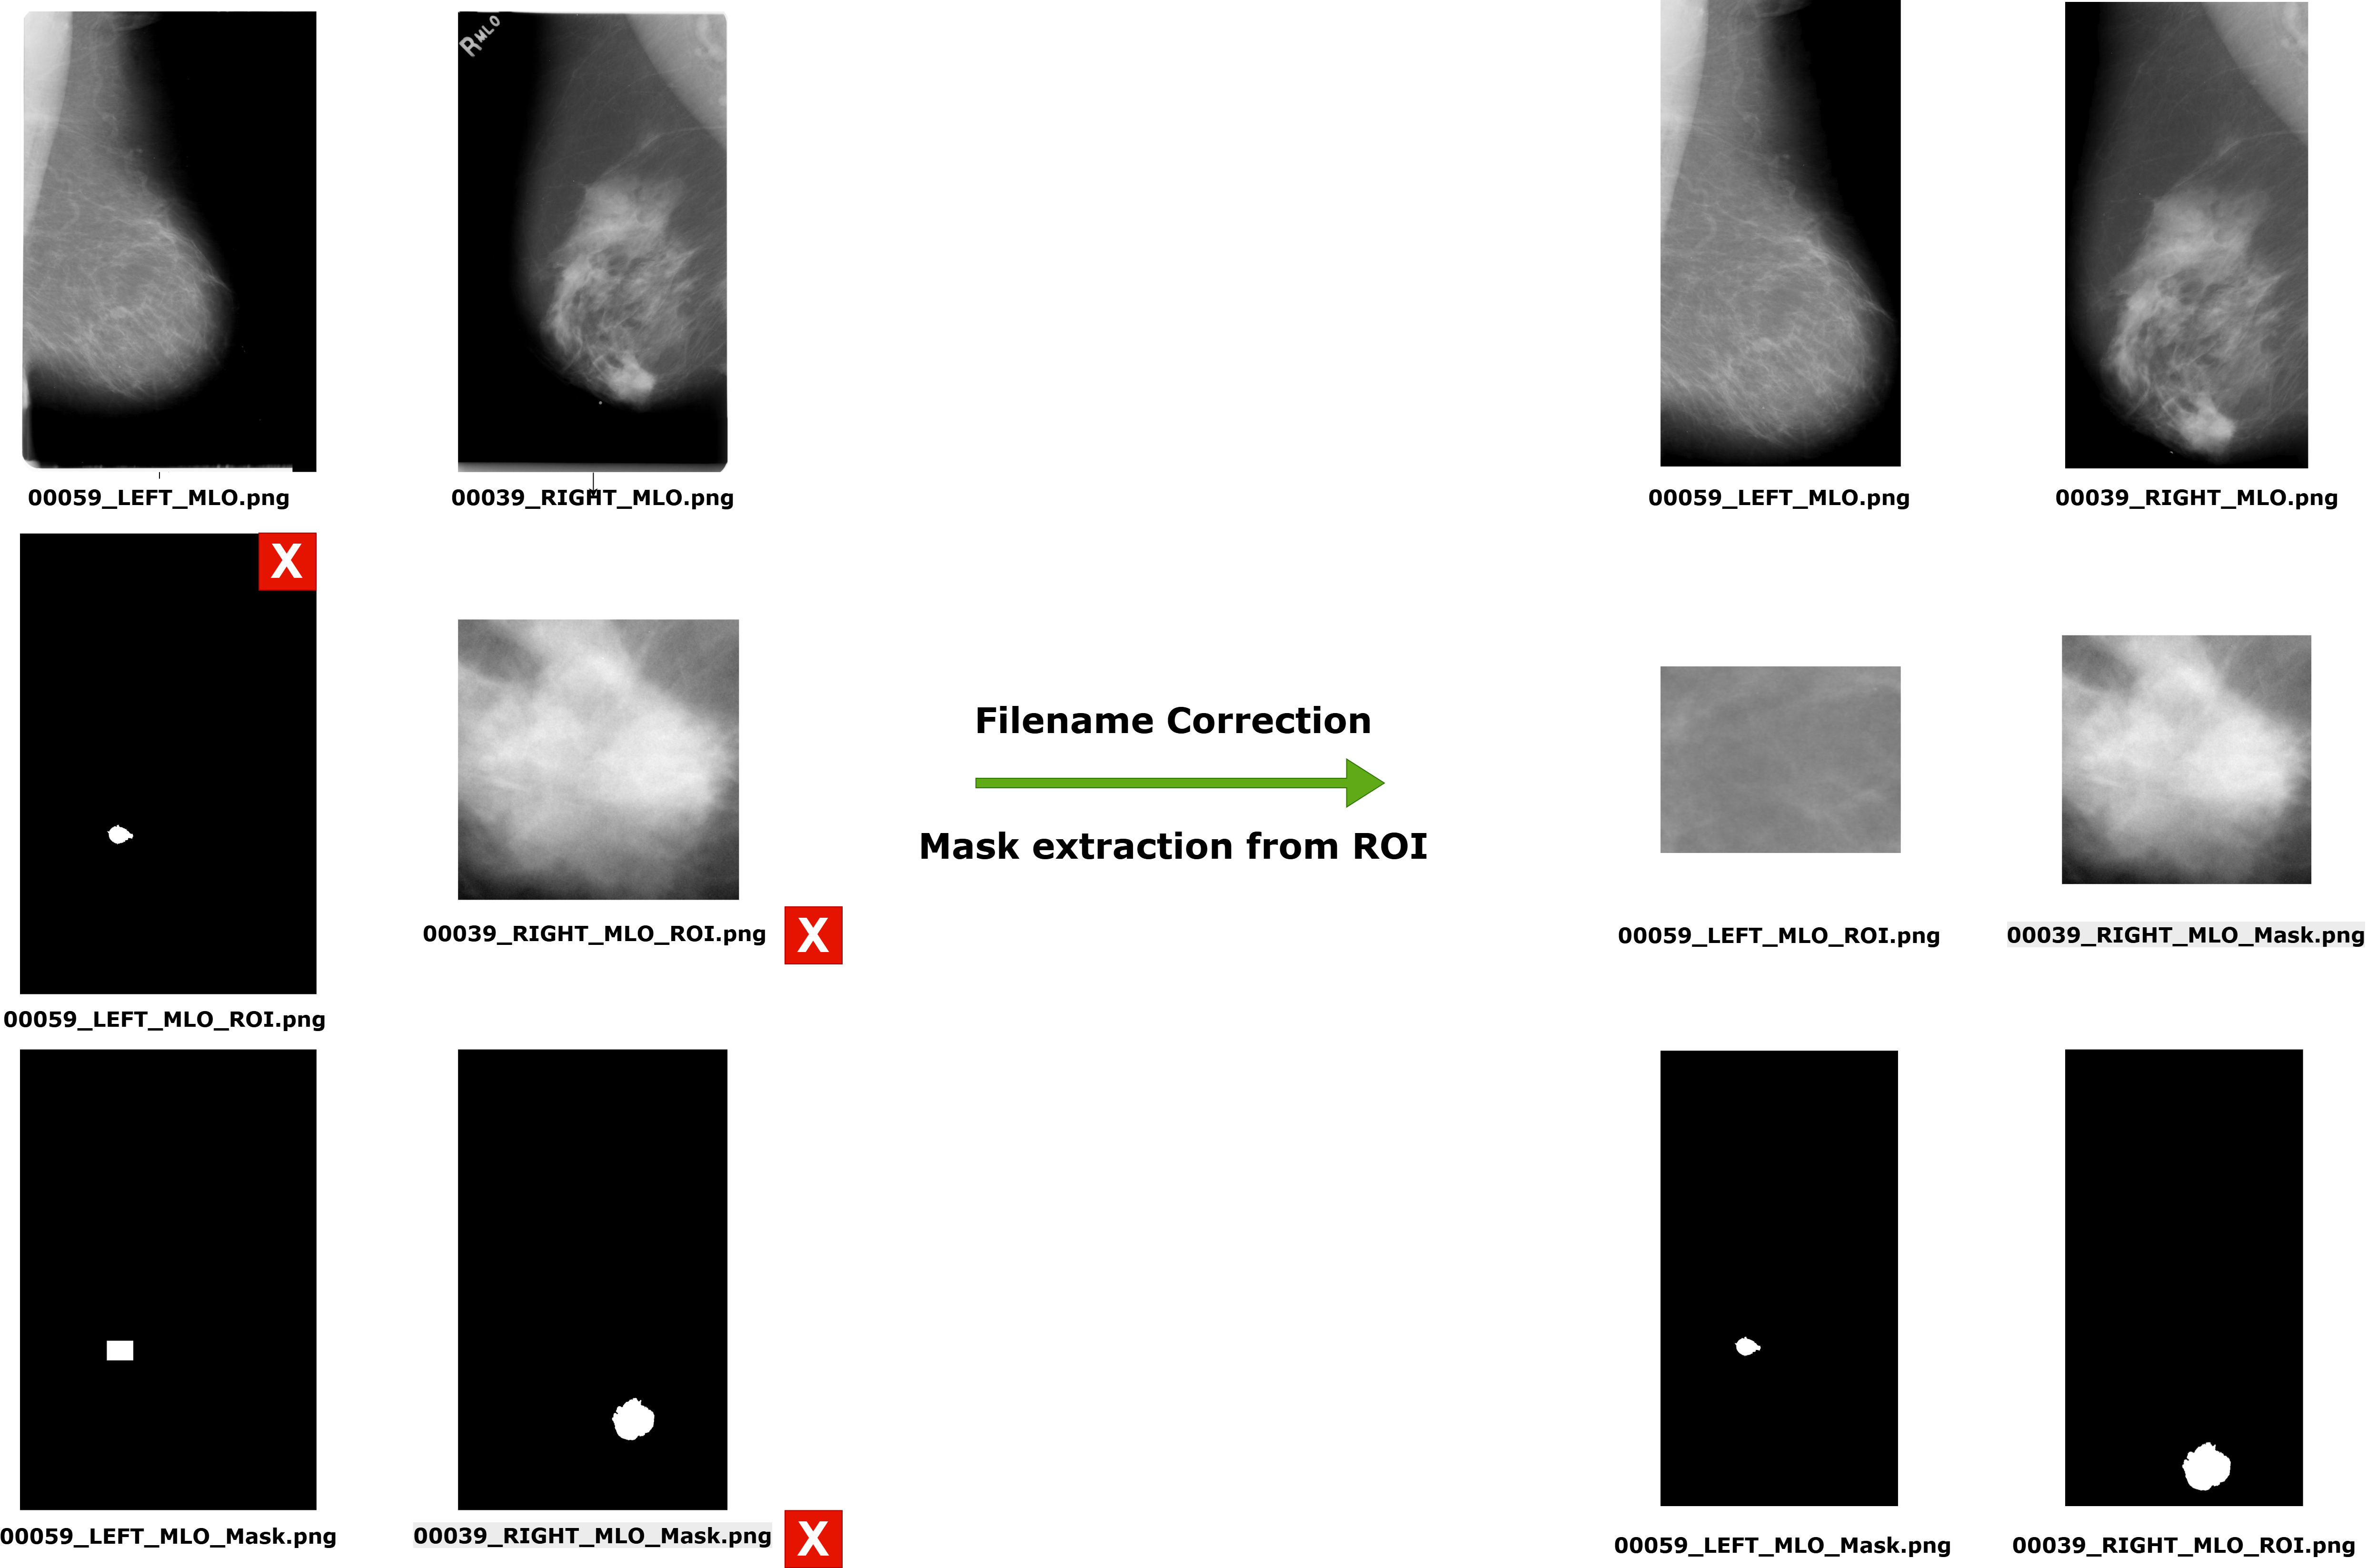
\includegraphics[width=0.5\linewidth]{preprocessing2.png}
        \end{figure}
    
\end{frame}

%--------

\begin{frame}{More about MaskRCNN}
\framesubtitle{Threshold Optimization optimization and Trade-offs}
    \begin{columns}
        \column{0.5\textwidth}
        \begin{figure}
            \centering
            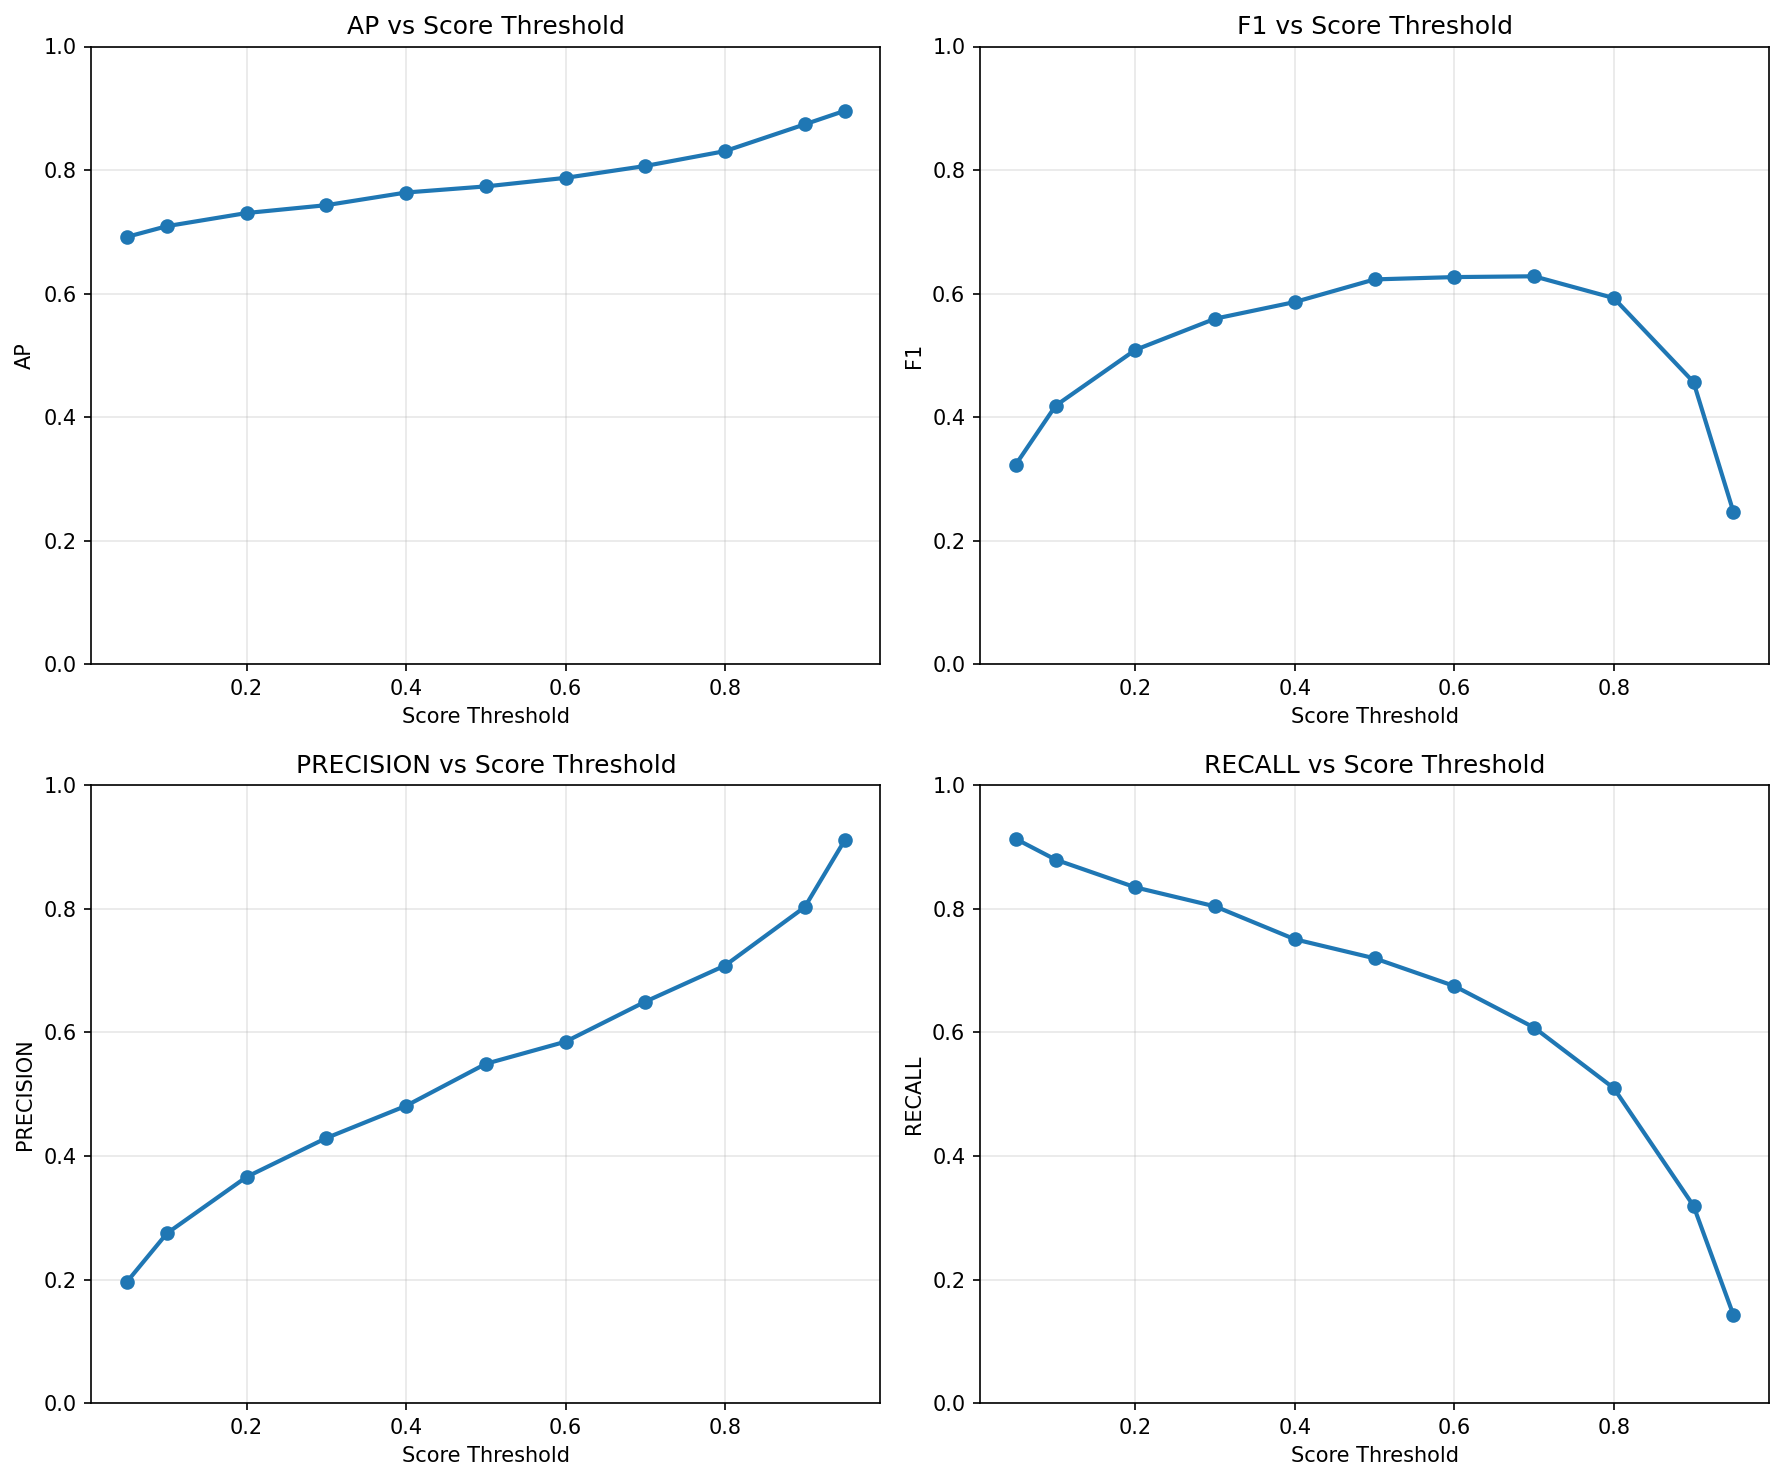
\includegraphics[width=0.85\linewidth]{metrics_vs_threshold.png}
            \caption{Performance metrics vs. confidence threshold}
        \end{figure}
        
        \column{0.5\textwidth}
                \begin{itemize}
            \item \textbf{Optimal Threshold:} 0.7 (F1-maximized)
            \item \textbf{F1-Score:} 0.62
            \item \textbf{Precision:} 0.65
            \item \textbf{Recall:} 0.6
            \item \textbf{High-confidence predictions:} 23.2\% above 0.5
        \end{itemize}
        
        \vspace{0.5cm}
        \begin{block}{Clinical Relevance}
            Threshold can be adjusted based on screening vs. diagnostic priorities
        \end{block}
    \end{columns}
\end{frame}

\begin{frame}{More about MaskRCNN}
\framesubtitle{Anchor Configuration Validation}
    \begin{columns}
        \column{0.5\textwidth}
        \begin{figure}
            \centering
            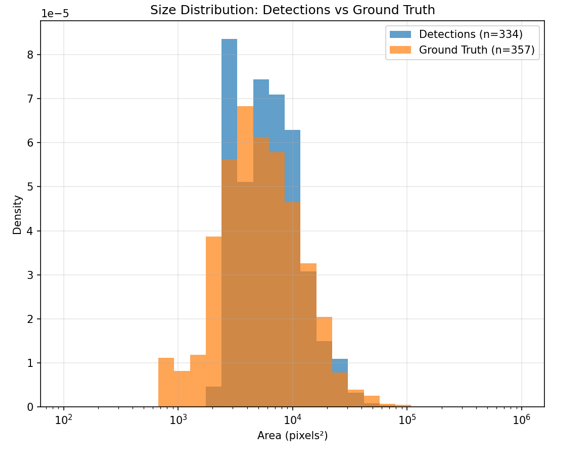
\includegraphics[width=\linewidth]{size_distribution.png}
            \caption{Predicted vs. ground truth size distributions}
        \end{figure}
        
        \column{0.5\textwidth}
        \begin{itemize}
            \item \textbf{Detected masses:} 334
            \item \textbf{Ground truth:} 357
            \item \textbf{Size range:} $10^3-10^5$ pixels²
            \item Close distribution alignment
        \end{itemize}
        
        \vspace{0.5cm}
        \begin{block}{Validation}
             No bias toward large/small masses\\
             Successful transfer learning\\
        \end{block}
    \end{columns}
\end{frame}
